\documentclass{article}
\usepackage{graphicx} % Required for inserting images
\usepackage[margin=1in]{geometry}
\usepackage{amsmath}
\usepackage{amsthm}
\usepackage{amssymb}
\usepackage{amsfonts}
\usepackage{enumitem}
\usepackage{verbatim}
\usepackage{xcolor}

\title{Homework 2: Report}
\author{Dante Buhl}
\date{April. $29^{th}$ 2024}


\DeclareMathOperator{\cond}{cond}
\DeclareMathOperator{\vecspan}{span}

\begin{document}

\newcommand{\bs}[1]{\boldsymbol{#1}}
\newcommand{\bmp}[1]{\begin{minipage}{#1\textwidth}}
\newcommand{\emp}{\end{minipage}}
\newcommand{\R}{\mathbb{R}}
%\newcommand{\Imag}{\mathbb{I}}
\newcommand{\C}{\mathbb{C}}
\newcommand{\N}{\mathcal{N}}
\newcommand{\I}{\mathrm{I}}
\newcommand{\K}{\bs{\mathrm{K}}}
\newcommand{\m}{\bs{\mu}_*}
\newcommand{\s}{\bs{\Sigma}_*}
\newcommand{\dt}{\Delta t}
\newcommand{\tr}[1]{\text{Tr}(#1)}
\newcommand{\Tr}[1]{\text{Tr}(#1)}
      
\maketitle

\section*{Problem 1: Absolute Stability for AB3}
\begin{enumerate}[label=\alph*)]

  \item Determine the largest value of $\Delta t$, for which the three-step 
        Adams-Bashforth method (AB3)
    \begin{proof}
      We use the condition for absolute stability: 
      \begin{align}
        \lim_{k \to \infty} ||\bs{u}_k|| = 0
      \end{align}
      For this specific numerical method, we have the following characteristic
      polynomial for the numerical method. (Note that since the columns of $B$
      are linearly independent we have that $B$ is diagonalizable).
      \begin{align}
        \bs{u}_{k+3} = \bs{u}_{k+2} + \frac{\dt}{12}\left(23\bs{f}_{k+2} -
        16\bs{f}_{k+1} + 5\bs{f}_k\right)\\
        \bs{u}_{k+3} - \bs{u}_{k+2} = \frac{\dt}{12}\left( 23\bs{Au}_{k+2} -
        16\bs{Au}_{k+1} + 5\bs{Au}_k\right)\\
        \bs{w}_{k+3} - \bs{w}_{k+2} = \frac{\dt}{12}\Lambda\left( 23\bs{w}_{k+2} -
        16\bs{w}_{k+1} + 5\bs{w}_k\right)
      \end{align}
      From this form of the Adams Bashforth method, we have that the
      coefficients $\alpha_i$ and $\beta_i$ are as follows, 
      \begin{align}
        \bs{\alpha} = [0, 0, -1, 1], \quad \bs{\beta} = \left[ \frac{5}{12},
        -\frac{16}{12}, \frac{23}{12}, 0\right]  \\
        \sum_{i=0}^3 (\alpha_i - \dt\lambda_m\beta_i)\bs{w}_{k+i}^m = 0
      \end{align}
      At this point, bother to find the eigenvalues of the matrix A which form
      $\Lambda$. Using a matlab eigenvalue solver, we find the eigenvalues of
      $A$ to be, 
      \begin{align*}
            \lambda \approx \left[ -0.9667 \pm i 30.1255, -99.0667\right]\\
            \R(\lambda) \approx \left[ -0.9667, -99.0667\right]
      \end{align*}
      We also only consider the real part of $\lambda$ as this is what will
      contribute to the convergence/stability. At this point we have 2 equations
      to solve in order to find the requirement on $\dt$ for the absolute
      convergence. The two equations are related to the characteristic
      polynomial for the iteration process. 
      \begin{align*}
        \pi(z) = \rho(z) - \dt\lambda_i\sigma(z) = 0\\
        \rho(z) = \sum_{j=0}^{q} \alpha_j z^j, \quad 
        \sigma(z) = \sum_{j=0}^{q} \beta_j z^j \\
        \rho(z) = z^3 - z^2, \quad \sigma(z) = \frac{23z^2 - 16z + 5}{12}
      \end{align*}   
      \begin{align}
        \pi(z)=0, \implies \dt = \frac{\rho(z)}{\lambda_i \sigma(z)}
      \end{align}
      This equation now becomes a constrained optimization problem. We consider
      two constraints. First, the value of $\dt$ must be a real value. We notice
      that the equation given to solve for $\dt$ is composed of three complex
      quantities, so there is no guarantee that the obtained value for $\dt$ is
      real. Second, we notice that the eigenvalues of the system that we wish to
      be a contraction must be of absolute value less than 1. That is, $|z| <
      1$. Therefore, we have two constraints, on a 3 variable optimization
      problem. We obtain three equations. 
      \begin{align}
        z = x + iy, \quad |z| < 1 &\implies x^2 + y^2 < 1\\
        \mathbb{I}(\dt) = 0 &\implies \mathbb{I}\left(\frac{\rho(x,
        y)}{\sigma(x, y)}\right) = 0\\
        \max \R(\dt) &\implies \nabla_h \R\left(\frac{\rho(x, y)}{\sigma(x,
        y)}\right) = \vec{0}
      \end{align}
      \begin{align*}
        \rho(x, y) &= x^3 - 3xy^2 - x^2 + y^2 + i\left(3x^2y - y^3 - 2xy\right)\\
        \sigma(x, y) &= \frac{23x^2 - 23y^2 -16x + 5 + i\left(46xy -16y\right)}{12}
      \end{align*}
      \begin{align*}
        \frac{\rho(x,y)}{\sigma(x,y)} &=
        \frac{\rho(x,y)\overline{\sigma}(x,y)}{|\sigma(x,y)|^2}\\
        \R\left(\frac{\rho(x,y)}{\sigma(x,y)}\right) &=
        \frac{\R\left(\rho(x,y)\overline{\sigma}(x,y)\right)}{|\sigma(x,y)|^2}\\
        \mathbb{I}\left(\frac{\rho(x,y)}{\sigma(x,y)}\right) &=
        \frac{\mathbb{I}\left(\rho(x,y)\overline{\sigma}(x,y)\right)}{|\sigma(x,y)|^2}\\
      \end{align*}
      The actual function beign considered here is quite unpleasant to write
      out explicitly. So the rest of this problem will proceed by the result of
      numerical work. The easiest way to solve this problem is as it is put in
      the notes. We consider the boundary of the domain for the eigenvalue, $z$,
      that will yield a contraction. This is of course the unit circle, $z =
      e^{i\theta}$. Then, we find the region of absolute stability from
      $\frac{\rho(e^{i\theta})}{\sigma(e^{i\theta})}$.
      \begin{center}
        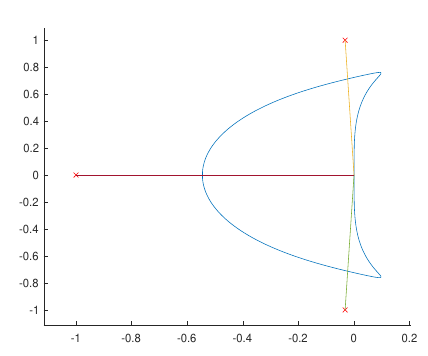
\includegraphics[width=0.6\textwidth]{1bStabRegion.png}
      \end{center}
      This yields a plot on the
      complex plane with eigenvalues that satisfy the problem we wish to solve.
      Then we overplot the normalized eigenvalues from our original matrix A, and draw
      lines originating from the origin to the eigenvalues of A in the complex
      plane. In order to ensure that $\dt$ is a real-valued, we must pick points
      on the region of absolute stability which are colinear with the
      eigenvalues of $A$. Then we determine the maximum $\dt$ by the ratio
      between the distance from the eigenvalue to the origin and the distance
      from the point colinear on the boundary of the region of absolute
      stability to the origin. This is then our $\dt$. We find for this problem,
      that the eigenvalue, $\lambda = -99.0667$ is furthest from the region of
      absolute stability, and appropriate $\dt$ for this eigenvalue is very
      close to $\dt = 0.00550593$. 
    \end{proof}
  \item 

\end{enumerate}


\section*{Question 2: Convergence and Asbolute Stability for the BDF3 Method}

Criterion for Consistency for a linear multistep method
\begin{align}
\rho(1) &=0 \\
\rho(1) - \sigma(1) &=0
\end{align}

\begin{enumerate}[label=\alph*)]

  \item       

\end{enumerate}
\section*{Question 3: Consistency, Convergence, and Stability for an LMM}

\section*{Question 4: Convergence and Stability for an RK Method}


\end{document}
